\begin{figure*}[t]
  \centering
  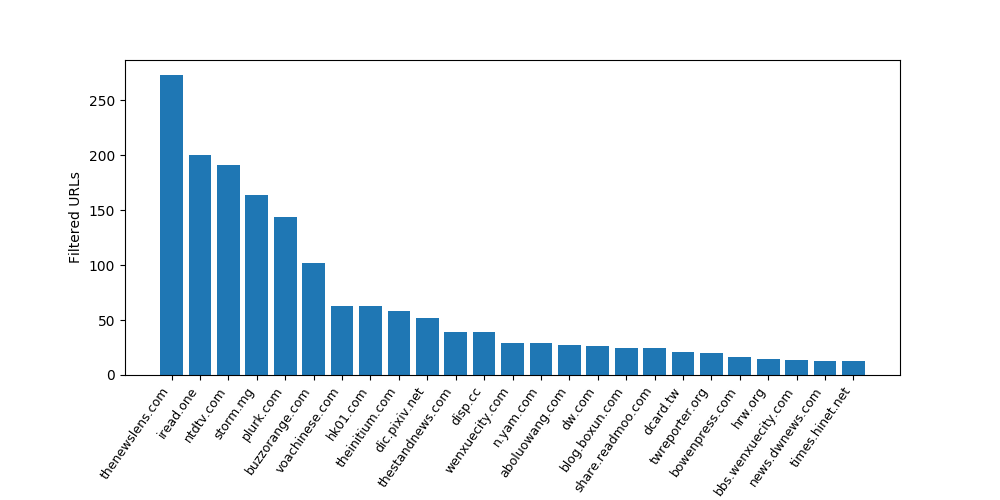
\includegraphics[scale=0.6]{figures/top-domains}
  \caption{\label{top-domains}Top censored domains by URL count.}
\end{figure*}

\section{Evaluation}

We performed a large-scale evaluation of our approach to
discover region-specific websites that are censored in China.  We
began by seeding with the Citizen Lab block list, which is
the most widely used list by censorship researchers. The list contains
220 web pages that either are blocked or have been alleged to be blocked in
the past. Since we only extract phrases from web pages that are
currently censored, we began by testing each web page on the block list for
censorship. This left us with 108 unique web pages and 85 domains.

From November 11th, 2017 to July 9th, 2018, we used Bing's Search API
to search for websites related to known censored
websites~\cite{microsoft:bing}. According to the API, each call can
return at most 50 search results. Since it would be expensive to
perform multiple API calls for each search term, we limited ourselves
to one API call, i.e. 50 search results, per search term. For each
website in the search results, we tested for censorship by sending a
DNS request to a set of controlled IP addresses in China that don't
belong to DNS servers. As with FilteredWeb, if we received a DNS
response, we inferred that the DNS request was intercepted, and thus
the tested website is censored. Finally, we performed three separate
evaluations to measure the effectiveness of different phrase sizes for
finding censored websites. With each evaluation, we only extracted
unigrams, bigrams, and trigrams, respectively. We also limited each
evaluation to 1,000,000 URLs to be consistent with the methodology of
FilteredWeb~\cite{darer2017filteredweb}.

We also configured the Bing API calls so that any URLs from Blogspot,
Facebook, Twitter, YouTube, and Tumblr would be ignored. We did this
for a couple of reasons. For one, these websites are widely known to
be censored in China, so we would not be providing new information by
having these websites or their subdomains in our result
set. Furthermore, Tumblr and Blogspot assign a unique subdomain to
each user's blog, and in some cases we'd get a dozen blogs from a
single search query. In order to find culture-specific websites that
are normally buried by the top 50 search results, then, we need to
omit these blogs.